\documentclass[12pt]{report}
\usepackage[utf8]{inputenc}

% no word splitting
\tolerance=1
\emergencystretch=\maxdimen
\hyphenpenalty=10000
\hbadness=10000

% every section on a new page
\usepackage{titlesec}
\newcommand{\sectionbreak}{\clearpage}

\usepackage{bm}

% includegraphics
\usepackage{graphicx}

% matrices signs
\usepackage{amsmath}
\usepackage{commath}

\begin{document}
The second order differential equation to solve is the following
$$\ddot{x}=\frac{1}{\rho r_0 R_{max}}\left [(P_i(t)-P_o(t))\cdot r_0-M(x)-D\frac{h_0}{r_0}\dot{x}\right ]\,,$$
where
$$M(x)=E\frac{h_0}{r_0}x \ , x>x^*$$
$$M(x)=4 \frac{E}{\pi^2}\cdot\frac{h_0^2}{r_0^2}\cdot\frac{h_0}{h_0+r_0+x}x \ , x\leq x^*$$
Let's say
\begin{equation}
y=\begin{pmatrix}y_1\\y_2\end{pmatrix}=\begin{pmatrix}x\\\dot{x}\end{pmatrix}
\label{eq:1}
\end{equation}
Then the derivative of $y$ would be

\begin{equation}
\dot{y}=\begin{pmatrix}\dot{y_1}\\\dot{y_2}\end{pmatrix}=\begin{pmatrix}\dot{x}\\\ddot{x}\end{pmatrix}
\label{eq:2}
\end{equation} 
So we can conclude the equation below.
\begin{equation} \dot{y}=\begin{pmatrix}\dot{x}\\\ddot{x}\end{pmatrix}=\begin{pmatrix}y_2\\\frac{1}{\rho r_0 R_{max}}\left [(P_i(t)-P_o(t))\cdot r_0-M(y_1)\cdot y_1-D\frac{h_0}{r_0}y_2\right ]\end{pmatrix}
\label{eq:3}
\end{equation} 

\begin{figure}[h]
	\centering
	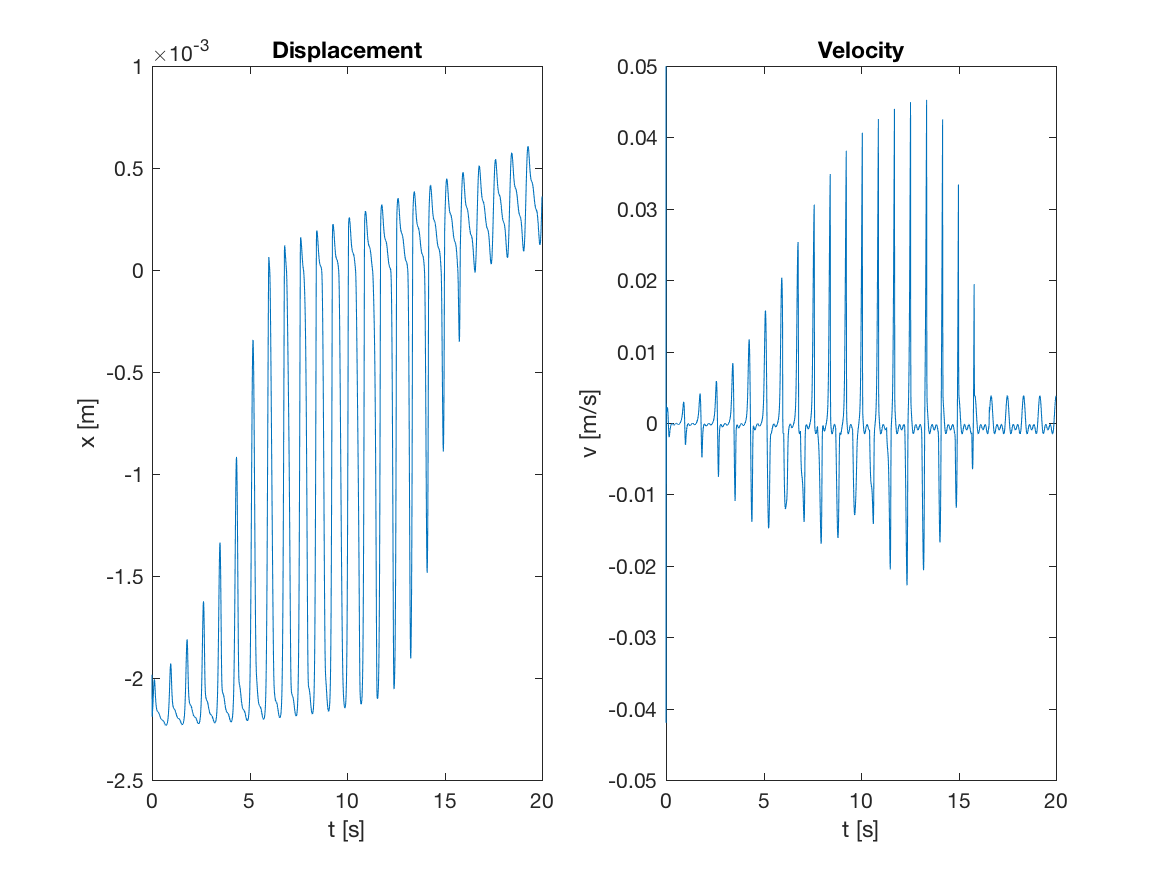
\includegraphics[width=15cm]{Pics/DispVeloEuler.png}
	\caption{Displacement and velocity for the first 20 seconds with Explicit Euler ($h = 0.0001$)}
	\label{fig:1}
\end{figure}

\begin{figure}[h]
	\centering
	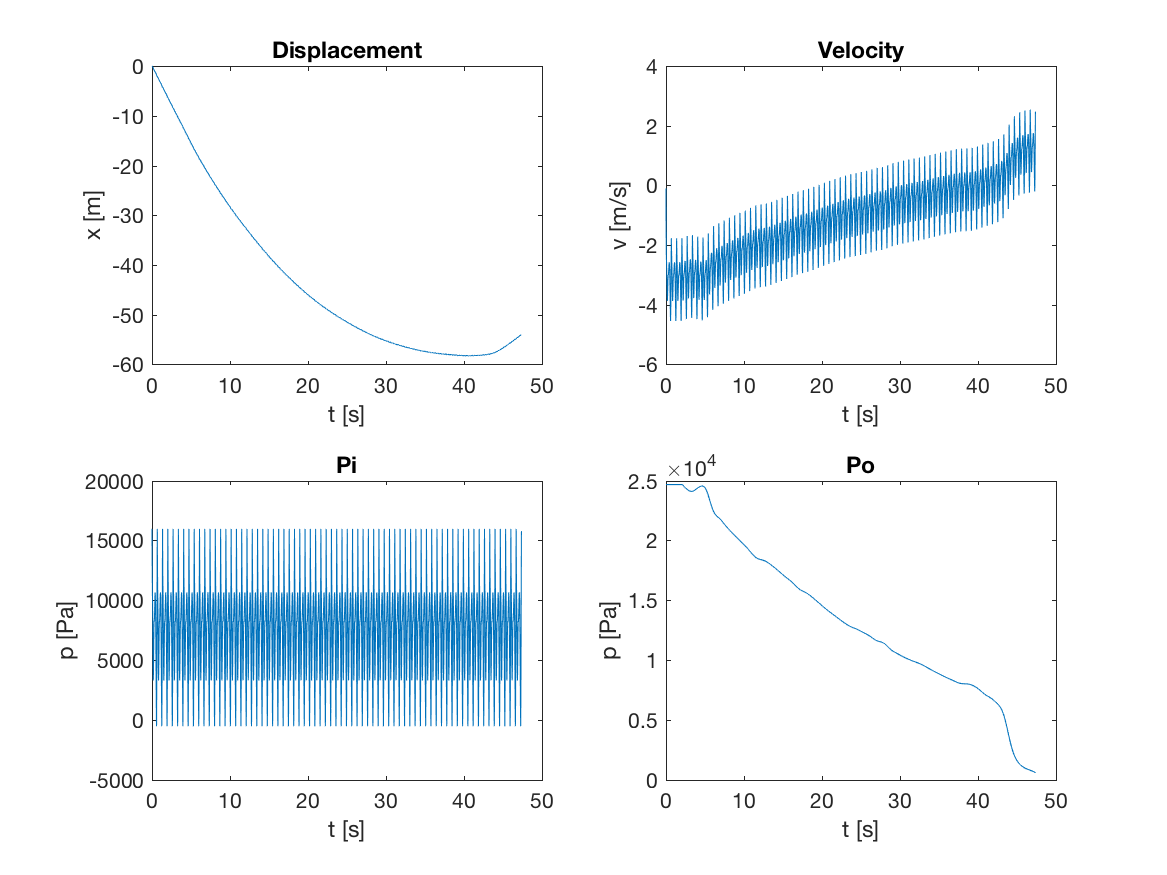
\includegraphics[width=15cm]{Pics/DispVeloRK4.png}
	\caption{Displacement and velocity for the first 20 seconds with Runge Kutta 4 ($h = 0.001$)}
	\label{fig:1}
\end{figure}
\end{document}